\section{Introduction And Motivation}
Blockchain is distributed ledger technology defined as "blah blah"
\subsection{Introduction To Blockhain}
\textit{“Blockchain is a continuously growing list of records, called blocks, which are linked and secured using cryptography. Each block contains typically a hash pointer as a link to a previous block, a timestamp and transaction data”} \cite{wiki:001}. It can serve as a distributed ledger that can record transactions without a central server or trusted third party. The transactions are available to all parties and are easily verifiable. It is inherently resistant to data tampering as altering data in any one block breaks the chain and requires that all subsequent blocks be calculated again using the new data. Technical details of blockchains are discussed in chapter [\ref{Blockchain}], however for a high level overview please refer to Figure \ref{fig:blockchain}. Blockchain has the power to revolutionize how business is conducted in digital age. Some are calling it the most important innovation since the development of the internet and the world wide web. The proponents of this technology believe that it will fundamentally transform the web itself. Internet of tomorrow will be powered by decentralized applications or Dapps. The first blockchain was invented by a person or group of persons known only by the pseudonym Satoshi Nakamoto. Bitcoin is a form of peer-to-peer electronic cash designed to transfer value between two parties without involving banks or other financial institutions. It was the first to solve the double spend problem in digital currency. Bitcoin paved the way for exponential growth in crypto currency market which together with other alt coins is worth over 120 billion dollars. The underlying technology which powers Bitcoin, Ethereum and other crypto currencies can be used for much more than just transferring X amount of crypto from Person A to Person B. Researchers are employing blockchain technologies to increase efficiency and reduce costs in industries such as Supply Chain Management, Internet of things, Banking and Finance.

%\ref{fig:PCIe}.\\
\begin{figure}[b]
	\centering
    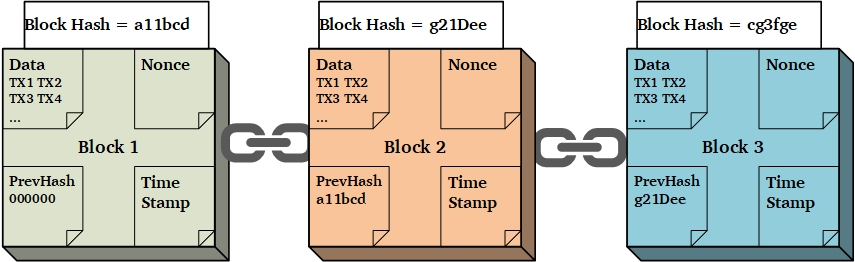
\includegraphics[width=160mm,scale=0.5]{figs/blockchain}
	\caption{High Level Overview of the Blockchain}
	\label{fig:blockchain}
\end{figure}
  
\subsection{Permissioned Vs Permission less blockchains vs Private blcokchain}
i.e. properties of each , reasons for each one to exist
https://github.com/ramxis/Thesis/blob/master/Miscellaneous/Recommended/bank-2020---blockchain-powering-the-internet-of-value---whitepaper.pdf use permissioned and permssioneless table from this paper as a guiding inspiration

\subsection{Motivation}
Thesis motivation text goes here....
Motivation, relevance, goals, research questions, hypotheses\ldots
\subsection{Thesis Objective}
objective.....
